%SParameters.tex
%
\documentclass[10pt,letterpaper,twoside,titlepage]{book}%
\title{S-Parameters}
\author{MA~Laforge}%
\def\AMSFooterTag{MA Laforge: S-Parameters}
\usepackage[singlespacing]{../Common/LaforgeDocStyle}%
%
\usepackage{graphicx}\graphicspath{{./figures/}}%
\usepackage{IEEEtrantools}%
\usepackage{amsmath}%
\usepackage{latexsym}%Provides the \Box command (for sheet resistance)
\usepackage[reim_shrthnd,reim_curly]{../Common/CustomCommands}%
%\usepackage[reim_symb,reim_round]{CustomCommands}%
\usepackage[sort,compress,noadjust]{cite}%Does not work for some reason
\usepackage{../Common/Hyphenation}%correct bad hyphenation here
%
%Custom commands:
%SParameters_CustCmds.tex
%Defines document-level custom commands
%
%Constants
%------------------------------------------------------------------------------
\newcommand{\maxfigwidth}{3.15in}%
%
%Equation alignment
%------------------------------------------------------------------------------
\newcommand{\EAtwocols}[4]{%
%Defines a 2-column line format for use in IEEEeqnarray.
%Output format:
%   [    #1][#2                 ][    #3][#4                 ]
%      w1        (1-w1)/2-w2        w2         (1-w1)/2
\parbox[t]{.15\linewidth}{\hfill\begin{IEEEeqnarraybox*}[][t]{r}#1\end{IEEEeqnarraybox*}}%
\parbox[t]{.35\linewidth}{\begin{IEEEeqnarraybox*}[][t]{l}#2\end{IEEEeqnarraybox*}}%
\parbox[t]{.075\linewidth}{\hfill\begin{IEEEeqnarraybox*}[][t]{r}#3\end{IEEEeqnarraybox*}}%
\parbox[t]{.425\linewidth}{\begin{IEEEeqnarraybox*}[][t]{l}#4\end{IEEEeqnarraybox*}}%
}%
%Matrix builders
%------------------------------------------------------------------------------
%Generate n-row column matrix using ellipsis:
%   nRowColMx{VAR}{SUBSCRIPT}{ROWVAR}
\newcommand{\nRowColMx}[3]{
	\left[\begin{IEEEeqnarraybox*}[][c]{,c,}
		#1_{{#2}1}\\#1_{{#2}2}\\\vdots\\#1_{{#2}{#3}}
	\end{IEEEeqnarraybox*}\right]
}
%Generate n-by-n *diagonal* matrix using ellipsis:
%   nRowColMx{VAR}{SUBSCRIPT}{DIAGVAR}
\newcommand{\nXnDiagMx}[3]{
	\left[\begin{IEEEeqnarraybox*}[][c]{,c/c/c/c,}
		#1_{{#2}1}&0&\cdots &0\\
		0&#1_{{#2}2}&\cdots &0\\
		\vdots &\vdots &\ddots &\vdots\\
		0&0&\cdots &#1_{{#2}{#3}}
	\end{IEEEeqnarraybox*}\right]
}
%Generate n-by-n matrix using ellipsis:
%   nRowColMx{VAR}{SUBSCRIPT}{ROWVAR}{COLVAR}
\newcommand{\nXnMx}[4]{
	\left[\begin{IEEEeqnarraybox*}[][c]{,c/c/c/c,}
		#1_{{#2}11}&#1_{{#2}12}&\cdots &#1_{{#2}1{#4}}\\
		#1_{{#2}21}&#1_{{#2}22}&\cdots &#1_{{#2}2{#4}}\\
		\vdots &\vdots &\ddots &\vdots\\
		#1_{{#2}{#3}1}&#1_{{#2}{#3}2}&\cdots &#1_{{#2}{#3}{#4}}
	\end{IEEEeqnarraybox*}\right]
}
%Figure boxes
%------------------------------------------------------------------------------
\newcommand{\columnbox}[1]{\parbox{\maxfigwidth}{#1}}%
\newcommand{\figsidebyside}[2]{\begin{figure}[!ht]\centering{#1}\quad{#2}\end{figure}}%
%Last Line

%
%
\begin{document}%
\frontmatter%The stuff following this command is before the main text (will have Roman page numbering, etc.)
%
\mainmatter%The stuff following this command is the main text (will have Arabic page numbering, etc.)
%ChSParams.tex
%
%------------------------------------------------------------------------------
\chapter{Scattering Parameters}
%------------------------------------------------------------------------------
\par Scattering parameters are a powerful analysis tool, providing much insight on the electrical behavior of circuits and devices at, and beyond microwave frequencies. Most vector network analyzers are designed with the built-in capability to display $S$ parameters. To an experienced engineer, $S$ parameter plots can be used to quickly identify problems with a measurement. A good understanding of their precise meaning is therefore essential. \emph{Talk about philosophy behind these derivations in order to place reader into context. Talk about how the derivations will valid for arbitrary complex reference impedances (once everything is hammered out). Talk about the view of pseudo-waves and the mocking of waveguide theory mentionned on p.\ 535 of \cite{pr:Marks_1992}. Talk about alterantive point of view where $S$-parameters are a conceptual tool that can be used to look at real traveling waves, but don't have to. Call pseudo-waves: traveling waves of a conceptual measurement setup. Is the problem of connecting a transmission line of different $Z_\mathrm{C}$ than was used for the measurement that it may alter the circuit's response (ex: might cause different modes to propagate), and thus change the network?? Question: forward/reverse scattering parameters: Is that when the input (port 1) is excited, or simly incident vs. reflected/transmitted???}
%
\par The reader is referred to \cite{bk:Collin_1992}\cite{pr:Marks_1992}\cite{bk:Pozar_2005} for a more general treatment, including non-TEM modes. \emph{Verify this statement, and try to include this if possible.}
%
%-------------------------------------------------------------------------------
\subsubsection{Traveling Waves And Pseudo-Waves}
%-------------------------------------------------------------------------------
\par Verify the following statements with the theory in \cite{pr:Marks_1992}.
\par Link to: Scattering and pseudo-scattering matrices.
\par Traveling waves: for applications where we are interrested in the real power traveling down a transmission line (ex: Calibration Techniques). Are these not also \emph{power waves???}
\par Pseudo-waves: for applications where the network itself is to be characterised, but measurement/propagation environment is not important.
\par Ideal $Z_\mathrm{0}=50\Ohm$ pseudo-waves are also used for system-level analyses under the premise that the transmission lines attached to the $S$-parameter network under study can be approximated as lossless lines of the same impedance.
%
%ChSParams_Formulate.tex
%
%------------------------------------------------------------------------------
\section{Network Characterization}
%------------------------------------------------------------------------------
%-------------------------------------------------------------------------------
\subsection{Low Frequency Solutions}
%-------------------------------------------------------------------------------
\begin{figure}[!ht]
	\centering
	\columnbox{
		\centering
		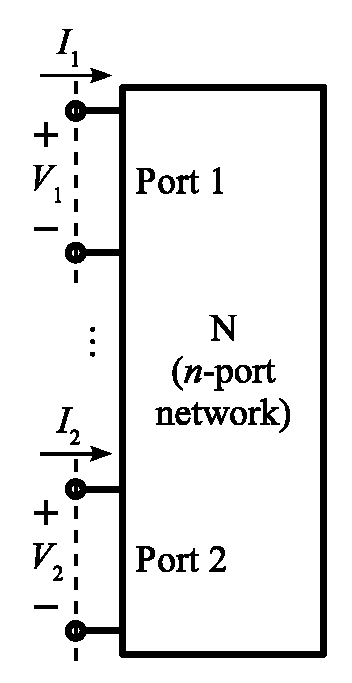
\includegraphics[scale=0.5]{NPortNetwork}
		\caption{Arbitrary linear $n$-port network, N.}
\label{fig:LinearTwoPortNetwork}%###############################################
	}%end\columnbox
	\quad
	\columnbox{
		\centering
		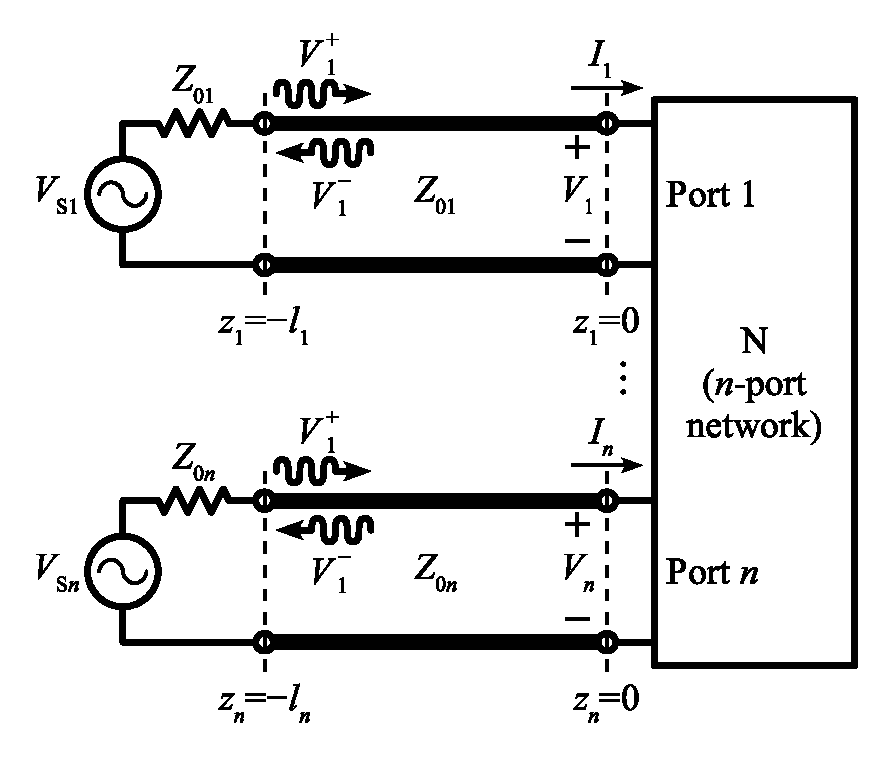
\includegraphics[scale=0.5]{SParamMeasSetup}
		\caption{Conceptual setup used to measure the $n$-port network. Note that both the the source impedances ($Z_{\mathrm{S}i}$) and characteristic impedances ($Z_{\mathrm{C}i}$) are set to a real, frequency independant reference impedance of $Z_{0i}$.}
\label{fig:SParamMeasSetup}%####################################################
	}%end\columnbox
\end{figure}
%
\par One of the commonly used and well understood network parameter types is the $Z$ parameters. For an $n$-port network (Fig.~\ref{fig:LinearTwoPortNetwork}) the $\matrixsymbol{Z}$ matrix relates terminal voltages as a function of terminal currents:
\begin{IEEEeqnarray}{rl}
	\matrixsymbol{V}&{}=\matrixsymbol{ZI}
\label{eq:ZPMatrixEquation}\\%##################################################
	\nRowColMx{V}{}{n}&{}=\nXnMx{z}{}{n}{n}\nRowColMx{I}{}{n}
	\textrm{.}
\end{IEEEeqnarray}
%
\par Conceptually, it is very simple to measure $Z$ parameters:
\begin{equation}
	z_{ij}=\left.\frac{V_i}{I_j}\right|_{I_k=0\textrm{, }\forall k\neq j}
	\textrm{.}
\end{equation}
%
\begin{itemize}%[\setlabelwidth{M)}]
	\item[1)]Inject a test current at port $j$, while leaving all remaining ports open-circuited ($I_k=0$, $\forall k\neq j$).
	\item[2)]Measure the voltages that develop at all terminals ($V_i$, $\forall i$).
	\item[3)]Repeat for all ports $j=1\ldots n$.
\end{itemize}
%
%-------------------------------------------------------------------------------
\subsection{High Frequency Limitations}
%-------------------------------------------------------------------------------
\par In general, it is not simple to apply a given current directly to a port, or measure the resulting voltage. The problem is that signals can only be applied and measured through some form of medium such as cables, which are represented as transmission lines in Fig.~\ref{fig:SParamMeasSetup}. At low frequencies, the cable parasitics, which are predominantly resistive losses, can often be ignored. \emph{Mention that we assume a single mode of propagation for each terminal pair: TEM. Does it matter that it is TEM, or just that there is a single mode?} However, in the general case, the solutions to the telegrapher's equations reveal that, at a given frequency, two distinct waves traveling in opposite directions can propagate the cables used for the measurement. The following expression relates net voltages and currents to traveling waves as a function of position on the cables:
\begin{IEEEeqnarray}{c}
	V_i(z_i)=V^+_i(z_i)+V^-_i(z_i)=V^+_{0i}e^{-\gamma_i z_i}+V^-_{0i}e^{\gamma_i z_i}
\label{eq:LossyTLineV}%########################################################
	\\I_i(z_i)=I^+_i(z_i)-I^-_i(z_i)=\frac{V^+_{0i}}{Z_{Ci}}e^{-\gamma_i z_i}-\frac{V^-_{0i}}{Z_{Ci}}e^{\gamma_i z_i}
\label{eq:LossyTLineI}%########################################################
	\textrm{,}
\end{IEEEeqnarray}
%
where
\begin{itemize}%[\setlabelwidth{}]
	\item[]$\gamma_i$ is the propagation constant of line $i$.
	\item[]$Z_{Ci}$ is the characteristic impedance of line $i$.
	\item[]$V_i(z_i)$ is the net voltage phasor at position $z_i$ of line $i$,
	\item[]$I_i(z_i)$ is the net current phasor flowing in the positive direction at position $z_i$ of line $i$,
	\item[]$V^+_i(z_i)$ is the voltage phasor of the traveling wave propagating in the positive direction at position $z_i$ of line $i$,
	\item[]$V^-_i(z_i)$ is the voltage phasor of the traveling wave propagating in the negative direction at position $z_i$ of line $i$,
	\item[]$V^+_{0i}\defAs V^+_i(0)$, and $V^-_{0i}\defAs V^-_i(0)$ are the incident and transmitted/reflected voltage phasors at port $i$ of N respectively.
\end{itemize}
%
\par Thus, at sufficiently high frequencies, the signal applied/measured at the input of the cables will no longer be adequately describe the X at the port interface. Moreover, it would also be impractical, if not impossible, to create open circuit conditions at high frequencies to perform a measurement. At certain frequencies, ``open-circuit'' conditions will simply behave as a connection to a mismatched transmission medium, allowing a non-negligeable amount of power to radiate from the port. In other cases, circuits might even become unstable if certain ports are left open-circuited.
%
%-------------------------------------------------------------------------------
\subsection{Traveling Wave Matrix}
%-------------------------------------------------------------------------------
\par The conceptual solution to high-frequency characterization is to provide a matched environment where networks are driven and loaded using perfectly terminated transmission lines ($Z_{\mathrm{S}i}=Z_{\mathrm{C}i}$) that represent the operating conditions. In reality, nonlinear loads, process variations, and other non-idealities only make it possible to approximate the operating conditions. However, if the measurement and operating environments are controlled within acceptable tolerances, it is possible to avoid disasterous situations such as oscillaiton conditions.  The resultant measurement should therefore adequately represent the microwave network.
%
\par A matched environment is only part of the solution. Network measurements performed remotely through cables must eventually be referenced to the port interfaces. This subject will be discussed in further detail in Chapter X. For the moment, it will simply be stated that a practical representation of high-frequency networks relates forward traveling waves, to the reverse traveling wave phasors at the port interfaces ($z_i=0$). This relationship is defined by the traveling wave matrix, $\matrixsymbol{S}^\mathrm{TW}$:
%
\begin{IEEEeqnarray*}{rl}
	\matrixsymbol{V}_0^-
	&{}=\matrixsymbol{S}^\mathrm{TW}\matrixsymbol{V}_0^+\IEEEyesnumber
\label{eq:TWMatrix_Definition}%#################################################
\\
	\nRowColMx{V^-}{0}{n}&{}=\nXnMx{s^\mathrm{TW}}{}{n}{n}\nRowColMx{V^+}{0}{n}\IEEEyesnumber
\label{eq:TWMatrix_ExpandedDef}%################################################
	\textrm{.}
\end{IEEEeqnarray*}
%
\par In order to compute $\matrixsymbol{S}^\mathrm{TW}$, degenerate versions of \eqref{eq:LossyTLineV} and \eqref{eq:LossyTLineI} will be used to restrict the analysis to the port interfaces:
\begin{IEEEeqnarray}{l}
\EAtwocols
	{V_i}{{}\defAs V_i(0)=V^+_{0i}+V^-_{0i}}
	{I_i}{{}\defAs I_i(0)=\frac{V^+_{0i}}{Z_{\mathrm{C}i}}-\frac{V^-_{0i}}{Z_{\mathrm{C}i}}
	\textrm{,}}
\end{IEEEeqnarray}
%
which can be expressed more succinctly in matrix form:
\begin{IEEEeqnarray*}{l}
\EAtwocols
	{\matrixsymbol{V}}{{}=\matrixsymbol{V}^+_0+\matrixsymbol{V}^-_0}
	{\matrixsymbol{I}}{{}=\matrixsymbol{Z}^{-1}_\mathrm{C}\left(\matrixsymbol{V}^+_0-\matrixsymbol{V}^-_0\right)}
\label{eq:TLineMatrix_PortInterface}%###########################################
\IEEEyesnumber\\
\EAtwocols
	{\nRowColMx{V}{}{n}}{{}=\nRowColMx{V^+}{0}{n}+\nRowColMx{V^-}{0}{n}}
	{\nRowColMx{I}{}{n}}{{}=\nXnDiagMx{Z^{-1}}{\mathrm{C}}{n}
		\left(\nRowColMx{V^+}{0}{n}-\nRowColMx{V^-}{0}{n}\right)}
\end{IEEEeqnarray*}
%
\par Note that $\matrixsymbol{Z}_\mathrm{C}$ is defined as:
%
\begin{equation}
	\matrixsymbol{Z}_\mathrm{C}
		\defAs\matrixsymbol{U}\nRowColMx{Z}{\mathrm{C}{n}}
		=\nXnDiagMx{Z}{\mathrm{C}}{n}
	\textrm{.}
\end{equation}
%
\par Substituting \eqref{eq:TLineMatrix_PortInterface} into \eqref{eq:ZPMatrixEquation}, each port ($i$) is implicitly connected to a transmission line of $\{Z_{Ci}, \gamma_i\}$:
\begin{IEEEeqnarray}{c}
	\matrixsymbol{V}^+_0+\matrixsymbol{V}^-_0
		=\matrixsymbol{ZZ}^{-1}_0(\matrixsymbol{V}^+_0-\matrixsymbol{V}^-_0)\nonumber\\
	(\matrixsymbol{ZZ}^{-1}_0+\matrixsymbol{U})\matrixsymbol{V}^-_0
		=(\matrixsymbol{ZZ}^{-1}_0-\matrixsymbol{U})\matrixsymbol{V}^+_0\nonumber\\
	\matrixsymbol{V}^-_0
		=(\matrixsymbol{ZZ}^{-1}_0+\matrixsymbol{U})^{-1}(\matrixsymbol{ZZ}^{-1}_0-\matrixsymbol{U})\matrixsymbol{V}^+_0
	\textrm{.}
\end{IEEEeqnarray}
%
\par Comparing with \eqref{eq:TWMatrix_Definition}, the traveling-wave matrix is given by:
\begin{equation}
	\matrixsymbol{S}^{\mathrm{TW}}=(\matrixsymbol{ZZ}^{-1}_0+\matrixsymbol{U})^{-1}(\matrixsymbol{ZZ}^{-1}_0-\matrixsymbol{U})
	\textrm{.}
\end{equation}
%
%-------------------------------------------------------------------------------
\subsubsection{Matrix Coefficient Measurement}
%-------------------------------------------------------------------------------
\par From \eqref{eq:TWMatrix_ExpandedDef}, the entries of $\matrixsymbol{S}^{TW}$ are given by:
\begin{equation}
	s_{ij}=\left.\frac{V^-_i}{V^+_j}\right|_{V^+_k=0\textrm{, }\forall k\neq j}
	\textrm{.}
\end{equation}
%
\par Thus, each entry $s_{ij}$ can be obtained from the ratio of the traveling wave voltage phasor emanating from port $i$ to the one incident to port $j$, when the incident waves at all other ports are of zero magnitude (non-existant). Fig.~\ref{fig:SParamMeasSetup} presents a simple setup allowing for the measurement of $s_{ij}$, assuming the availability of a mechanism detecting traveling waves at the port interfaces:
\begin{itemize}%[\setlabelwidth{M)}]
	\item[1)]Excite network N with source $V_{\mathrm{S}j}$, while leaving all remaining sources off ($V_{\mathrm{S}k}=0$, $\forall k\neq j$).
	\item[2)]Measure the voltage phasor of the incident wave at port $j$, and that of the transmitted/reflected waves at all ports $i$ ($V^+_j$, and $V^-_i$, $\forall i$).
	\item[3)]Repeat for all ports $j=1\ldots n$.
\end{itemize}
%
\par Since both the transmission line characteristic impedance and the generator source impedance are equal to the (real) reference impedance of the port ($Z_{\mathrm{S}i}=Z_{\mathrm{C}i}=Z_{0i}$), all waves emanating from the excited network will be fully dissipated by the source impedances. This ensures that no component of the transmitted/reflected waves reflect back to violate the condition $V^+_k=0$, $\forall k\neq j$. Alternatively, the ports not being excited ($k\neq j$) can be terminated by a simple impedance of $Z_{\mathrm{T}i}=Z_{0i}$ instead of a transmission line. The voltage developed at the terminals of $Z_{\mathrm{T}i}$ would correspond to $V^-_i$. It should be emphasized that the measurement setup is conceptual, and would only be practical in a simulation environment. Real-world, $S$-parameter measurements are performed using devices called reflectometers\cite{pr:Engen_1979}\cite{pr:Eul_1991}, which are critical components of network analyzers. Mathematical calibration techniques then translate the measurements to the proper reference planes, at the port interfaces \cite{pr:Marks_1992}.
%
%-------------------------------------------------------------------------------
\subsubsection{Power of Traveling Waves}
%-------------------------------------------------------------------------------
\par\emph{\cite{bk:InanInan_1998}page 150.  Also in other book.}
\par In terms of node voltages and currents, the power delivered (derive? cite?) to a load is given by:
\begin{IEEEeqnarray}{c}
	P=\frac{1}{2}\realS{V\cdot I^*}%
	=\frac{1}{2}\real{V\cdot\left(\frac{V}{Z}\right)^*}
	\\=\frac{1}{2}\frac{V\cdot V^*}{\realS{Z}}
	\textrm{,{\qquad}since }V\cdot V^*\elemSpace{R}%\in\Re
	\textrm{.}
\end{IEEEeqnarray}
%
\par A similar expression can be obtained for the power transported by individual traveling waves on transmission line $i$ (justify?):
%
\begin{IEEEeqnarray*}{l}
\EAtwocols
	{P^+_i}{{}\defAs\textrm{Incident power}}
	{P^-_i}{{}\defAs\textrm{Transmitted/reflected power}}
\\\EAtwocols
	{P^+_i}{{}=\frac{1}{2}\frac{V^+_{i}\cdot V^{+*}_{i}}{\realS{Z_{0i}}}}
	{P^-_i}{{}=\frac{1}{2}\frac{V^-_{i}\cdot V^{-*}_{i}}{\realS{Z_{0i}}}\textrm{.}}
	\IEEEyesnumber
\label{eq:IncTransReflPower}%###################################################
\end{IEEEeqnarray*}
%
\par I am not sure if this is correct.  MUST BE CONFIRMED. Show how this relates to the power loss due to the attenuation on the line? (Power lost should be equivalent to change in transported power at 2 different points on the line).
%
%-------------------------------------------------------------------------------
\subsection{Normalized $S$ Parameters}
%-------------------------------------------------------------------------------
\par From a circuit analysis perspective, the concept of de-coupling a network from its measurement setup or real operating environment is a non-issue.  Consequently, it should be possible to use any set of transmission lines with their associated $Z_{\mathrm{C}i}$, and $\gamma_i$ to perform a measurement. Although
$Z_{Ci}\defAs Z_{0i}$
\par When comparing quantities, it is often easier to cast them onto a more meaningful form. In consequence, microwave engineers almost always work with \emph{normalized} scattering parameters, which are readily transformed into more meaningful quantities: incident and transmitted/reflected \emph{powers}. However, the main reason normalized scattering parameters are preferred is because they ensure that the matrices of reciprocal networks are symmetrical \cite{bk:Collin_1992}.
%
\par Let us define $\matrixsymbol{a}$ and $\matrixsymbol{b}$ as $n$-by-1 column matrices:
\begin{equation}
	\matrixsymbol{a}\defAs\matrixsymbol{Z}^{-\frac{1}{2}}_0\matrixsymbol{V}^+_0
	\textrm{,\quad and\quad}
	\matrixsymbol{b}\defAs\matrixsymbol{Z}^{-\frac{1}{2}}_0\matrixsymbol{V}^-_0
\label{eq:abMatrixDef}%#########################################################
	\textrm{,}
\end{equation}
%
where
\begin{equation}
	\matrixsymbol{Z}^{-\frac{1}{2}}_0
	=\left[\begin{IEEEeqnarraybox*}[][c]{,c/c/c/c,}
		\sqrt{Z_{01}}^{-1}&0&\cdots &0\\
		0&\sqrt{Z_{02}}^{-1}&\cdots &0\\
		\vdots &\vdots &\ddots &\vdots\\
		0&0&\cdots &\sqrt{Z_{0n}}^{-1}
	\end{IEEEeqnarraybox*}\right]
	\textrm{.}
\end{equation}
%
\par Thus, matrices $\matrixsymbol{a}$ \& $\matrixsymbol{b}$ hold \emph{normalized} incident and transmitted/reflected voltage phasors of the traveling waves:
\begin{equation}
	a_i=\frac{V^+_{0i}}{\sqrt{Z_{0i}}}
	\textrm{,\quad and\quad}
	b_i=\frac{V^-_{0i}}{\sqrt{Z_{0i}}}
	\textrm{.}
\end{equation}
%
\par Since the normalized quantities $a_i$ \& $b_i$ account for the characteristic impedance of their respective lines, they are more closely related to the incident and transmitted/reflected powers than their counterparts $V^+_i$ \& $V^-_i$:
\begin{IEEEeqnarray*}{l}
\EAtwocols
	{P^+_i}{{}=\frac{1}{2}a_i\cdot a^*_i}
	{P^-_i}{{}=\frac{1}{2}b_i\cdot b^*_i}
\IEEEyesnumber\\
\EAtwocols
	{P^+_i}{{}=\frac{1}{2}\frac{V^+_{0i}\cdot V^{+*}_{0i}}{\sqrt{Z_{0i}}\cdot\sqrt{Z_{0i}}^*}}
	{P^-_i}{{}=\frac{1}{2}\frac{V^-_{0i}\cdot V^{-*}_{0i}}{\sqrt{Z_{0i}}\cdot\sqrt{Z_{0i}}^*}\textrm{.}}
\end{IEEEeqnarray*}
%
\par\emph{ERROR: This does not correspond to the power of the traveling-wave matrix because $\realS{Z_{0i}}\neq\sqrt{Z_{0i}}\cdot\sqrt{Z_{0i}}^*$. This might be why $\{a_i, b_i\}$ appear to be defined differently in \cite{pr:Marks_1992}.}
%
\par If we isolate $\matrixsymbol{V}^+$ \& $\matrixsymbol{V}^-$ from \eqref{eq:abMatrixDef}:
\begin{equation}
	\matrixsymbol{V}^+=\matrixsymbol{Z}^\frac{1}{2}_0\matrixsymbol{a}
	\textrm{ and }
	\\\matrixsymbol{V}^-=\matrixsymbol{Z}^\frac{1}{2}_0\matrixsymbol{b}
	\textrm{,}
\end{equation}
%
we can substitute them in \eqref{eq:TLineMatrix_PortInterface}:
\begin{IEEEeqnarray}{c}
	\matrixsymbol{V}=\matrixsymbol{Z}^\frac{1}{2}_0(\matrixsymbol{a}+\matrixsymbol{b})
	\\\matrixsymbol{I}=\matrixsymbol{Z}^{-1}_0\matrixsymbol{Z}^\frac{1}{2}_0(\matrixsymbol{a}-\matrixsymbol{b})
		=\matrixsymbol{Z}^{-\frac{1}{2}}_0(\matrixsymbol{a}-\matrixsymbol{b})
	\textrm{,}
\end{IEEEeqnarray}
%
and, in turn, into \eqref{eq:ZPMatrixEquation}:
\begin{IEEEeqnarray}{c}
	\matrixsymbol{Z}^\frac{1}{2}_0(\matrixsymbol{a}+\matrixsymbol{b})
		=\matrixsymbol{ZZ}^{-\frac{1}{2}}_0(\matrixsymbol{a}-\matrixsymbol{b})\nonumber\\
	(\matrixsymbol{ZZ}^{-\frac{1}{2}}_0+\matrixsymbol{Z}^\frac{1}{2}_0)\matrixsymbol{b}
		=(\matrixsymbol{ZZ}^{-\frac{1}{2}}_0-\matrixsymbol{Z}^\frac{1}{2}_0)\matrixsymbol{a}\nonumber\\
	\matrixsymbol{b}=(\matrixsymbol{ZZ}^{-\frac{1}{2}}_0+\matrixsymbol{Z}^\frac{1}{2}_0)^{-1}
		(\matrixsymbol{ZZ}^{-\frac{1}{2}}_0-\matrixsymbol{Z}^\frac{1}{2}_0)\matrixsymbol{a}
	\textrm{.}
\end{IEEEeqnarray}
%
\par We now have an expression for the \emph{normalized} scattering matrix (in terms of $Z$ parameters), $\matrixsymbol{S}$, relating normalized transmitted/reflected waves to the incident waves:
\begin{equation}
	\matrixsymbol{b}=\matrixsymbol{Sa}
	\textrm{,}
\end{equation}
%
where
\begin{equation}
	\matrixsymbol{S}=(\matrixsymbol{ZZ}^{-\frac{1}{2}}_0+\matrixsymbol{Z}^\frac{1}{2}_0)^{-1}
		(\matrixsymbol{ZZ}^{-\frac{1}{2}}_0-\matrixsymbol{Z}^\frac{1}{2}_0)
\label{eq:MatrixZtoS}%##########################################################
	\textrm{.}
\end{equation}
%
\par This does not appear to correspond to p.\ 548 of \cite{pr:Marks_1992}. Find out why.
%
\par Isolating matrix $\matrixsymbol{Z}$ from this expression yields:
\begin{equation}
	\matrixsymbol{Z}=\matrixsymbol{Z}^\frac{1}{2}_0(\matrixsymbol{U}+\matrixsymbol{S})
		(\matrixsymbol{U}-\matrixsymbol{S})^{-1}\matrixsymbol{Z}^\frac{1}{2}_0
	\textrm{.}
\end{equation}
%
\par Given that $\matrixsymbol{Y}=\matrixsymbol{Z}^{-1}$, a relationship between $Y$ and $S$ parameters is also obtained:
\begin{IEEEeqnarray}{c}
	\matrixsymbol{S}=(\matrixsymbol{Y}^{-1}\matrixsymbol{Z}^{-\frac{1}{2}}_0+\matrixsymbol{Z}^\frac{1}{2}_0)^{-1}
		(\matrixsymbol{Y}^{-1}\matrixsymbol{Z}^{-\frac{1}{2}}_0-\matrixsymbol{Z}^\frac{1}{2}_0)
	\textrm{,}
	\\\textrm{and }\matrixsymbol{Y}=\matrixsymbol{Z}^{-\frac{1}{2}}_0(\matrixsymbol{U}-\matrixsymbol{S})
		(\matrixsymbol{U}+\matrixsymbol{S})^{-1}\matrixsymbol{Z}^{-\frac{1}{2}}_0
	\textrm{.}
\end{IEEEeqnarray}
%
%-------------------------------------------------------------------------------
\subsubsection{One-Port Matrix}
%-------------------------------------------------------------------------------
\par Note that, in the special case of a one-port matrix, \eqref{eq:MatrixZtoS} simplifies to:
\begin{IEEEeqnarray}{rl}
	s_{11}
		&=(z_{11}Z^{-\frac{1}{2}}_{01}+Z^\frac{1}{2}_{01})^{-1}
			(z_{11}Z^{-\frac{1}{2}}_{01}-Z^\frac{1}{2}_{01})
		\\&=\frac{z_{11}-Z_{01}}{z_{11}+Z_{01}}
	\textrm{,}
\end{IEEEeqnarray}
%
which can further be reduced by letting $Z\defAs z_{11}$ and $Z_0\defAs Z_{01}$:
\begin{equation}
	\Gamma\defAs s_{11}=\frac{Z-Z_0}{Z+Z_0}
	\textrm{.}
\end{equation}
%
\par The symbol $\Gamma$ is is often preferred to represent the reflection coefficient ($\Gamma\defAs{V^-}/{V^+}$) when only a single port is involved. In fact, all reflection coefficients, $s_{ii}$, correspond to a degenerate one port network:
\begin{equation}
	\Gamma_i\defAs s_{ii}=\frac{V^-_{i}}{V^+_{i}}
	\textrm{,}
\end{equation}
%
under the condition that all other ports ($k\neq i$) are terminated properly. The common factor of $\sqrt{Z_{0i}}$ in phasors $a_i$ and $b_i$ simply cancel out. Transmission coefficients ($s_{ij}$, where $i\neq j$) are slightly more complex quantities, especially if $Z_{0i}\neq Z_{0j}$.
%
%Last line
%
%ChSParams_Transmission.tex
%
%-------------------------------------------------------------------------------
\section{Scattering Transmission Parameters, $\matrixsymbol{T}$}
%-------------------------------------------------------------------------------
The scattering transmission matrix relates the normalized power waves in a form which computes the incident/reflected waves at port 1 as a function of those present at port 2:
\begin{equation}
	\left[\begin{IEEEeqnarraybox*}[][c]{,c,}
		b_{1}\\a_{1}%
	\end{IEEEeqnarraybox*}\right]
	=\left[\begin{IEEEeqnarraybox*}[][c]{,c/c,}
		t_{11}&t_{12}\\
		t_{21}&t_{22}%
	\end{IEEEeqnarraybox*}\right]
	\left[\begin{IEEEeqnarraybox*}[][c]{,c,}
		a_{2}\\b_{2}%
	\end{IEEEeqnarraybox*}\right]
	\textrm{.}
\end{equation}
%
The scattering transmission matrix is typically defined using $\matrixsymbol{T}$:
\begin{equation}
	\matrixsymbol{T}
	\defAs\left[\begin{IEEEeqnarraybox*}[][c]{,c/c,}
		t_{11}&t_{12}\\
		t_{21}&t_{22}%
	\end{IEEEeqnarraybox*}\right]
\end{equation}
%
Thus, the response for a cascade of networks can be computed from a simple matrix multiplication \emph{provided} the port 1 reference impedance of $\matrixsymbol{T}_{i+1}$ is equivalent to the port 2 reference impedance of $\matrixsymbol{T}_i$ (GENERATE FIGURE).
%
\subsubsection{Network Parameter Conversion ($\matrixsymbol{S}\Leftrightarrow\matrixsymbol{T}$)}
\par Taken from \cite{pr:Marks_1992} - have not confirmed whether correct - Derive?:
\begin{equation}
	\matrixsymbol{T}=\frac{1}{s_{21}}
	\left[\begin{IEEEeqnarraybox*}[][c]{,c"c,}
		s_{12}s_{21}-s_{11}s_{22}&s_{11}\\
		-s_{22}&1
	\end{IEEEeqnarraybox*}\right]
	\textrm{.}
\label{eq:StoT}%################################################################
\end{equation}
%
%------------------------------------------------------------------------------
\section{Cascade of 2 Transmission Line Segments}
\begin{figure}[!ht]
	\centering
	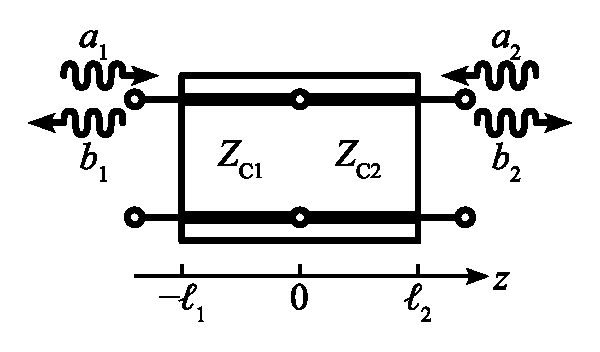
\includegraphics[scale=0.6]{ZCDiscontinuity}
	\caption{Cascaded transmission line segments.}
\label{fig:ZCDiscontinuity}%##################################################
\end{figure}
%
\par Consider the discontinuity in Fig.~\ref{fig:ZCDiscontinuity} formed by cascading transmission lines of different characteristic impedance values. Note that $z=0$ is now positionned at the discontinuity instead of the port interfaces. This notation will lead to a more elegant derivation of the network parameters.
%
\par Instead of using pseudo-waves, we will use traveling waves... TRY TO CONNECT SENTENCES. Next, consider the reference impedance of each port, $Z_\mathrm{01}$ and $Z_\mathrm{02}$ to respectively match these values, $Z_\mathrm{C1}$ and $Z_\mathrm{C2}$:
\begin{equation}
	Z_\mathrm{01}=Z_\mathrm{C1}
	\textrm{, and }
	Z_\mathrm{02}=Z_\mathrm{C2}
\label{eq:CascadedLines_Z0eqZC}%################################################
	\textrm{.}
\end{equation}
%
As a consequence, reflected waves will be fully absorbed by the port terminations during the conceptual $S$-parameter measurement that follows.  Given that the transmission lines are terminated with their respective $Z_{\mathrm{C}i}$, the forward \& reverse reflection coefficients at the interface of the discontinuity are given by (Fig.~\ref{fig:ZCDiscontinuity_Gamma}):
\begin{figure}[!ht]
	\centering
	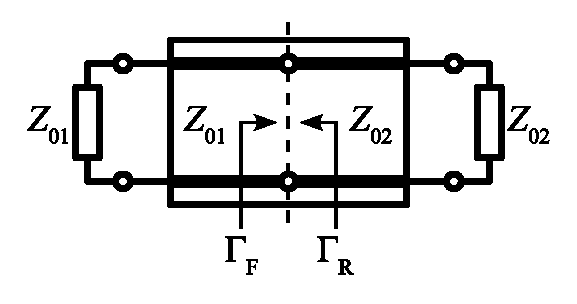
\includegraphics[scale=0.6]{ZCDiscontinuity_Gamma}
	\caption{Reflection coefficients at interface of perfectly terminated lines.}
\label{fig:ZCDiscontinuity_Gamma}%##################################################
\end{figure}
%
\begin{equation}
	\Gamma_\mathrm{F}= \frac{Z_\mathrm{02}-Z_\mathrm{01}}{Z_\mathrm{02}+Z_\mathrm{01}}
%\label{eq:ZPMatrixEquation}%###################################################
	\textrm{, and }
	\Gamma_\mathrm{R}= \frac{Z_\mathrm{01}-Z_\mathrm{02}}{Z_\mathrm{01}+Z_\mathrm{02}}
	\textrm{.}
\end{equation}
%
where
\begin{itemize}%[\setlabelwidth{}]
	\item[]Subscripts ``F", and ``R" identify quantities as ``forward" or ``reverse" reflection coefficients, respectively.
\end{itemize}
%
\subsubsection{Forward Transmission/Reflection}
\begin{figure}[!ht]
	\centering
	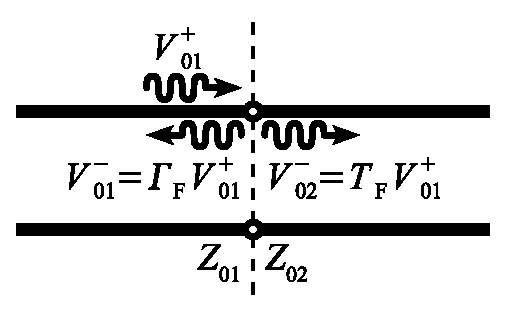
\includegraphics[scale=0.6]{ZCDiscontinuity_Forward}
	\caption{Forward transmission/reflection at the discontinuity.}
\label{fig:ZCDiscontinuity_Forward}%##################################################
\end{figure}
%
Next, consider the forward transmission/reflection (excitation at port 1 only) of a wave through the discontinuity (Fig.~\ref{fig:ZCDiscontinuity_Forward}). If $V^+_{01}$ defines the incident wave phasor at the discontinuity itself, position-dependent expressions for the incident, reflected and transmitted wave phasors are given by:
\begin{IEEEeqnarray}{rl}
	V_\mathrm{F}^\mathrm{I}(z)
		&{}=V^+_{01}e^{-{\gamma_1}z}
\label{eq:IncVoltAtZCDisc}%#####################################################
		\textrm{,}\\
	V_\mathrm{F}^\mathrm{R}(z)
		&{}=V^-_{01}e^{{\gamma_1}z}={\Gamma_\mathrm{F}}V^+_{01}e^{{\gamma_1}z}
\label{eq:ReflVoltAtZCDisc}%####################################################
		\textrm{,}\\\textrm{and }
	V_\mathrm{F}^\mathrm{T}(z)
		&{}={V^-_{02}}e^{{\gamma_2}z}=(V^+_{01}+V^-_{01})e^{-{\gamma_2}z}
		=(1+\Gamma_\mathrm{F})V^+_{01}e^{-{\gamma_2}z}
\label{eq:TransVoltAtZCDisc}%###################################################
	\textrm{.}
\end{IEEEeqnarray}
%
Thus, the forward transmission coefficient is defined as $T{\equiv}1+\Gamma_\mathrm{F}$.
%
\subsubsection{Power Conservation at the Discontinuity}
\par Verify power conservation.  Was not able to do so, but should work as follows.  Using \eqref{eq:IncTransReflPower} at the discontinuity ($z=0$):
\begin{IEEEeqnarray*}{rl}
	\textrm{incident power}
		&{}=\textrm{transmitted power}+\textrm{reflected power}\IEEEyesnumber\\
	P^\mathrm{I}_F
		&{}=P^\mathrm{T}_F+P^\mathrm{R}_F\\
	\frac{1}{2}\frac{V^\mathrm{I}_F\cdot V^{\mathrm{I}*}_F}{\realS{Z_{01}}}
		&{}=\frac{1}{2}\frac{V^\mathrm{T}_F\cdot V^{\mathrm{T}*}_F}{\realS{Z_{02}}}
		+\frac{1}{2}\frac{V^\mathrm{R}_F\cdot V^{\mathrm{R}*}_F}{\realS{Z_{01}}}\\
	\frac{1}{\realS{Z_{01}}}
			&{}=\frac{(1+\Gamma_\mathrm{F})\cdot(1+\Gamma_\mathrm{F})^*}{\realS{Z_{02}}}
			+\frac{\Gamma_\mathrm{F}\cdot \Gamma_\mathrm{F}^*}{\realS{Z_{01}}}
	\textrm{.}\IEEEyesnumber
\end{IEEEeqnarray*}
%
\subsubsection{Scattering Parameters}
\par The forward scattering parameters of the network in Fig.~\ref{fig:ZCDiscontinuity} can therefore be computed from the phasor values at the port interfaces:
\begin{IEEEeqnarray*}{l}
\EAtwocols
	{s_{11}}{
		{}=\left.\frac{b_1}{a_1}\right|_{a_2=0}
		=\frac{V_\mathrm{F}^\mathrm{R}(-\ell_1)/\sqrt{Z_{01}}}{V_\mathrm{F}^\mathrm{I}(-\ell_1)/\sqrt{Z_{01}}}
	}{s_{21}}{
		{}=\left.\frac{b_2}{a_1}\right|_{a_2=0}
		=\frac{V_\mathrm{F}^\mathrm{T}(\ell_2)/\sqrt{Z_{02}}}{V_\mathrm{F}^\mathrm{I}(-\ell_1)/\sqrt{Z_{01}}}
	}
\\\EAtwocols
	{\therefore s_{11}}{
		{}=\Gamma_\mathrm{F}e^{-2{\gamma_1}\ell_1}
	}{\therefore s_{21}}{
		{}=\frac{\sqrt{Z_{01}}}{\sqrt{Z_{02}}}(1+\Gamma_\mathrm{F})e^{-({\gamma_1}\ell_1+{\gamma_2}\ell_2)}
		\textrm{.}
	}\IEEEyesnumber
\end{IEEEeqnarray*}
%
\par By symmetry, and because $\Gamma_\mathrm{R}=-\Gamma_\mathrm{F}$, the reverse transmission coefficients are given by:
\begin{IEEEeqnarray*}{l}
\EAtwocols
	{s_{22}}{
		{}=\left.\frac{b_2}{a_2}\right|_{a_1=0}
		=\Gamma_\mathrm{R}e^{-2{\gamma_2}\ell_2}
	}{s_{12}}{
		{}=\left.\frac{b_1}{a_2}\right|_{a_1=0}
		=\frac{\sqrt{Z_{02}}}{\sqrt{Z_{01}}}(1+\Gamma_\mathrm{R})e^{-({\gamma_1}\ell_1+{\gamma_2}\ell_2)}
	}
\\\EAtwocols
	{\therefore s_{22}}{
		{}=-\Gamma_\mathrm{F}e^{-2{\gamma_2}\ell_2}
	}{\therefore s_{12}}{
		{}=\frac{\sqrt{Z_{02}}}{\sqrt{Z_{01}}}(1-\Gamma_\mathrm{F})e^{-({\gamma_1}\ell_1+{\gamma_2}\ell_2)}
		\textrm{.}
	}\IEEEyesnumber
\end{IEEEeqnarray*}
%
%------------------------------------------------------------------------------
\section{$S$-Parameter Reference Impedance Transformer}
\par The result of matching the $S$-parameter reference impedances of the cascaded transmission line segments to their respective line impedances in \eqref{eq:CascadedLines_Z0eqZC} is to reference the associated \emph{power waves} ($a_1$, $b_1$, $a_2$, and $b_2$) to those same impedances. This property can easily be leveraged to perform a transformation of reference impedances.
%
\par Consider a transmitter designed to drive a line of $Z_\mathrm{C}=Z_{0\mathrm{TX}}$. The simulated linear $S$-parameter model of the transmitter would typically be referenced to a (often real) frequency independant impedance, $Z_{0\mathrm{S}}$.  Conceptually, the output can be connected to pair of cascaded transmission lines with arbitrary characteristic impedances.  However, if the $Z_{01}$ connected to the driver output matches $Z_{0\mathrm{S}}$, the network cascade is more readily computed from the two $\matrixsymbol{T}$ matrices. Furthermore, if the length of both line segments are set to zero, the cascade of lines degenerates into an ideal thru, thus behaving as a perfect $Z_{01}:Z_{02}$ transformer. If $Z_{02}$ is then chosen to correspond to $Z_{0\mathrm{TX}}$, the resulting $\matrixsymbol{T}$-matrix will therefore be referenced to the physical \emph{traveling} waves $a^{'}_{\mathrm{TX}}$ \& $b^{'}_{\mathrm{TX}}$ GENERATE FIGURE.
%
\par The $\matrixsymbol{T}$-matrix of the impedance transformer is therefore obtained by substituting REF EQ for $\ell_1=\ell_2=0$ in \eqref{eq:StoT}:
\begin{IEEEeqnarray*}{l}
\EAtwocols
	{t_{11}}{{}=\left.\frac{s_{12}s_{21}-s_{11}s_{22}}{s_{21}}\right|_{\ell_1=\ell_2=0}}
	{t_{12}}{{}=\left.\frac{s_{11}}{s_{21}}\right|_{\ell_1=\ell_2=0}}
\\\EAtwocols
	{t_{21}}{{}=\left.\frac{-s_{22}}{s_{21}}\right|_{\ell_1=\ell_2=0}}
	{t_{22}}{{}=\left.\frac{1}{s_{21}}\right|_{\ell_1=\ell_2=0}\textrm{.}}
\end{IEEEeqnarray*}
%
Which yields:
\begin{equation}
	\matrixsymbol{T}=\frac{1}{1+\Gamma_\mathrm{F}}
	\frac{\sqrt{Z_{02}}}{\sqrt{Z_{01}}}
	\left[\begin{IEEEeqnarraybox*}[][c]{,c/c,}
		1&\Gamma_\mathrm{F}\\
		\Gamma_\mathrm{F}&1
	\end{IEEEeqnarraybox*}\right]
	\textrm{.}
%\label{eq:StoT}%################################################################
\end{equation}
%
\par Another interresting form is obtained by noting that $1+\Gamma_\mathrm{F}=\frac{2Z_{02}}{Z_{02}+Z_{01}}$:
\begin{equation}
	\matrixsymbol{T}=\frac{1}{2Z_{02}}
	\frac{\sqrt{Z_{02}}}{\sqrt{Z_{01}}}
	\left[\begin{IEEEeqnarraybox*}[][c]{,c/c,}
		Z_{02}+Z_{01}&Z_{02}-Z_{01}\\
		Z_{02}-Z_{01}&Z_{02}+Z_{01}
	\end{IEEEeqnarraybox*}\right]
	\textrm{.}
%\label{eq:StoT}%################################################################
\end{equation}
%
\par Note: This does not match eq.\ 79 of \cite{pr:Marks_1992}.  One of the reasons may have something to do with the fact the $Q^{nm}$ matrix is defined with $a_n$ \& $b_n$ rows reversed.  Note that eq.\ 79 also an extra term,  $\left|Z_{02}/Z_{01}\right|$. If we let $\sqrt{Z_{0i}}\defAs r_ie^{j\theta_i}$, we get:
%
\begin{IEEEeqnarray*}{rl}
	\left|\frac{Z_{02}}{Z_{01}}\right|
	&=\left|\frac{(r_2e^{j\theta_2})^2}{(r_1e^{j\theta_1})^2}\right|
	=\left|\frac{r^2_2e^{j2\theta_2}}{r^2_1e^{j2\theta_1}}\right|
	=\frac{r^2_2}{r^2_1}
	\textrm{.}
\end{IEEEeqnarray*}
\par I cannot explain this discrepancy.
%
%Last line%
%Last line%
%
\backmatter%Supposed to be called before the bibliography & index - I don't know why
%------------------------------------------------------------------------------
%Bibliography
%------------------------------------------------------------------------------
\bibliographystyle{IEEEtran}%
\cleardoublepage%Go to next page so that "\addcontentsline" points to the correct page
	\addcontentsline{toc}{chapter}{\bibname}%Add bibliography to table of contents
	\bibliography{IEEEfull,../Common/CustomStrings,../Common/ReferenceDB}%
%
\end{document}%
%Last line
